\textit{Portions of this chapter were originally published in collaboration with Rory Barnes, Rodrigo Luger, and Jacob VanderPlas in March 2020 in the Astrophysical Journal (\citet{Fleming2020}, ApJ, Vol. 891, 2; 2020 \textcopyright \ American Astronomical Society, DOI: 10.3847/1538-4357/ab77ad), and are reproduced below with permission of the American Astronomical Society.}

\

In this Chapter, I combine my theoretical models, Bayesian inference, and machine learning to build a probabilistic model for TRAPPIST-1's long-term X-ray and ultraviolet (XUV) luminosity evolution. I condition this model on observations of TRAPPIST-1, and their uncertainties, and infer model parameters using Markov Chain Monte Carlo (MCMC) sampling. I demonstrate that TRAPPIST-1 likely maintained high $L_{XUV}/L_{bol} \approx 10^{-3}$ throughout its lifetime and could still be in the saturated emission phase today. Given these constraints, I then estimate the evolving XUV radiation environment experienced by its planetary system and consider how this evolution could have impacted the volatile inventory of the TRAPPIST-1 planets. I explain how my modeling is too computationally-expensive to scale to additional systems or more complex models, motivating the use of novel machine learning methods to significantly reduce the computational cost. I apply the open-source Python machine learning package introduced in Chapter 5, \approxposterior, to this problem. I demonstrate how \approxposterior can accurately replicate my inference, but requires nearly three orders of magnitude fewer computational resources. This massive reduction in computational cost enables my approximate inference method to scale to new computationally-expensive research problems. 

%% Intro %%

\section{Introduction} \label{trap:sec:intro}

The James Webb Space Telescope (JWST) is poised to detect and characterize the first terrestrial exoplanet atmospheres via transmission spectroscopy. This search will likely focus on planets orbiting nearby M dwarfs given their favorable relative transit depths, the potential buildup of biosignature gases due to UV-driven photochemistry \citep{Segura2005}, and the large occurrence rates of M dwarf planets \citep{Dressing2015}. The correct interpretation of those observations, however, is predicated on understanding the system's long-term evolution, most importantly processes that could impact the planet's atmospheric state and habitability, such as atmospheric escape, water loss, and the potential buildup of an abiotic O$_2$ atmosphere \citep{Watson1981,Lammer2003,MurrayClay2009,Luger2015}. These volatile escape mechanisms are partially driven by the host star's XUV luminosity (X-ray and EUV emission ranging over approximately 1-1000\AA), and therefore characterizing the long-term stellar XUV evolution of late M-dwarfs is critical to assessing the present state of their planets, including habitability.

High-energy stellar radiation originates from the corona via the heating of magnetically-confined plasma \citep{Vaiana1981}. The stellar magnetic field is likely generated via differential rotation within the stellar convective envelope \citep{Parker1955}, linking rotation to stellar activity and XUV emission. Stellar rotation rates slow over time due to magnetic braking \citep{Skumanich1972}, causing XUV emission to decline with time. The X-ray luminosity ($L_{X}$) of FGK stars, for example, has been empirically shown to monotonically decrease with age \citep{Jackson2012}. This trend has also been observed for commonly-used proxies for stellar age, rotation period and Rossby number \citep[Ro = $P_{rot}/\tau$ for convective turnover timescale $\tau$,][]{Pizzolato2003,Wright2011}. 

Stellar activity evolution is characterized by two distinct phases. First, in the saturated phase, young, rapidly-rotating stars ($\mathrm{Ro}\lsim 0.1$) maintain a constant $L_{X}/L_{bol} \approx 10^{-3}$ \citep{Wright2011,Jackson2012}. Then, at longer rotation periods and larger Ro, stars transition to the unsaturated phase in which $L_{X}/L_{bol}$ exponentially decays over time \citep{Pizzolato2003,Ribas2005}. Recent work has shown that the stellar dynamo processes that generate magnetic fields and drive XUV emission in fully-convective M dwarfs follow the same evolution with Ro as described above for solar-type stars \citep{Wright2016,Wright2018}. I can therefore apply this model to examine the XUV evolution of individual fully-convective stars.

TRAPPIST-1 \citep{Gillon2016,Gillon2017}, an ultracool dwarf located 12 pc from Earth, harbors 7 approximately Earth-sized transiting planets that are prime targets for JWST transmission spectroscopy observations \citep{Morley2017,Lincowski2018,Lustig2019}. TRAPPIST-1's high observed L$_{X}$ \citep{Wheatley2017}, short photometric rotation period \citep[3.3 d, ][]{Luger2017}, and low Rossby number \citep[Ro $\approx 0.01$, ][]{Roettenbacher2017} suggest that TRAPPIST-1 is still saturated today \citep{Pizzolato2003,Wright2011,Wright2018}. Both \citet{Roettenbacher2017} and \citet{Morris2018} suggest that the photometrically-determined rotation period is inaccurate, with the latter study proposing that the 3.3 d period corresponds to a characteristic timescale for active regions on the stellar surface. TRAPPIST-1's $v \sin i = 6$ km s$^{-1}$ \citep{Barnes2014}, however, implies a rotation period of ${\sim}1$ d for $i = 90^{\circ}$, providing evidence that TRAPPIST-1's rapid rotation is physical and consistent with saturation \citep[$P_{rot} \lsim 20$ d,][]{Wright2018}. 

The TRAPPIST-1 planetary system currently receives significant high-energy fluxes \citep{Bourrier2017b,Wheatley2017,Peacock2019}, possibly a consequence of TRAPPIST-1 remaining in the saturated regime. These fluxes were likely more extreme during the pre-main sequence, driving significant water loss and potentially rendering the planets uninhabitable \citep{Bolmont2017,Bourrier2017a}. Here, I model the long-term stellar and XUV evolution of TRAPPIST-1 to characterize the evolving XUV environment of its planetary system. I use MCMC to derive probability distributions for the model parameters that describe the XUV evolution that are consistent with TRAPPIST-1's observed properties and their uncertainties.

TRAPPIST-1 is not the only system that merits this modeling, however, as the Transiting Exoplanet Survey Satellite will likely discover additional transiting planets orbiting in the habitable zone of nearby M dwarfs \citep{Barclay2018}, some of which may be suitable targets for atmospheric characterization with JWST. In this work, I show that stellar XUV histories can be accurately inferred using machine learning \citep[\approxposterior, ][]{FlemingVanderPlas2018}, but using $980\times$ less computational resources than traditional MCMC methods. This speed-up enables my methods to scale to additional stars that host potential targets for atmospheric characterization and is generalizable to a large number of applications, potentially enabling Bayesian statistical analyses that are otherwise intractable with traditional MCMC approaches, e.g. \emcee \citep{ForemanMackey2013}.

I describe my model and statistical methods in $\S$~\ref{trap:sec:methods}. I present my results and demonstrate the ability of machine learning to reproduce the analysis in $\S$~\ref{trap:sec:results}, and discuss the implications of the results in $\S$~\ref{trap:sec:discussion}. In $\S$~\ref{AP:sec:app}, I describe the \approxposterior algorithm and discuss its convergence properties.

\section{Methods} \label{trap:sec:methods}

\subsection{Simulating XUV Evolution with \vplanet} \label{trap:sec:model}

I simulate TRAPPIST-1's stellar evolution using the \stellar module in \vplanet\footnote{\vplanet is publicly available at \href{https://github.com/VirtualPlanetaryLaboratory/vplanet}{https://github.com/VirtualPlanetaryLaboratory/vplanet}.} \citep{Barnes2019}, which performs a bicubic interpolation over mass and age of the \citet{Baraffe2015} stellar evolution tracks. The \citet{Baraffe2015} models (also employed by both \citet{Burgasser2017} and \citet{vanGrootel2018} to constrain TRAPPIST-1's stellar properties) were computed for solar metallicity stars and hence are suitable for TRAPPIST-1 whose [Fe/H] is consistent with solar \citep[][see also \citet{Burgasser2017}]{Gillon2016}.

I assume TRAPPIST-1's L$_{XUV}$ evolution traces that of L$_{X}$ and use the \citet{Ribas2005} model,
\begin{align}
\label{trap:eqn:lxuv}
\frac{L_\mathrm{XUV}}{L_\mathrm{bol}} = \left\{
				\begin{array}{lcr}
					f_\mathrm{sat} &\ & t \leq t_\mathrm{sat} \\
					f_\mathrm{sat}\left(\frac{t}{t_\mathrm{sat}}\right)^{-\beta_\mathrm{XUV}} &\ & t > t_\mathrm{sat}
				\end{array}
				\right.,
\end{align}
where $f_{sat}$ is the constant ratio of stellar XUV to bolometric luminosity during the saturated phase, $t_{sat}$ is the duration of the saturated phase, and $\beta_{XUV}$ is the exponent that controls how steeply L$_{XUV}$ decays after saturation. In practice, I define $f_{sat} = \log_{10}(L_{XUV}/L_{bol})$ and transform Eqn.~(\ref{trap:eqn:lxuv}) accordingly.

Note that each \vplanet simulation (and hence likelihood calculation, see $\S$~\ref{trap:sec:mcmc:like}) in principle only requires interpolating the \citet{Baraffe2015} $L_{bol}$ tracks and evaluating an explicit function of time to compute $L_{XUV}$, both computationally-cheap tasks. \vplanet, however, is a general purpose code designed to simulate the evolution of an exoplanetary system and its host star by simultaneously integrating coupled ordinary differential equations and explicit functions of time that describe the evolution. This generalized structure requires numerous steps to facilitate physical couplings, such as validation steps and a host of intermediate calculations \citep[for more details, see][]{Barnes2019}. Moreover, \stellar simultaneously evolves a star's radius, effective temperature, radius of gyration, $L_{XUV}$, and rotation rate in addition to $L_{bol}$, adding computational overhead. Each \vplanet simulation using \stellar therefore lasts about 10s.

% extra
% The L$_{X}$ evolution of fully-convective stars follows the same broken power law model examined for partially-convective FGK stars \citep{Wright2016,Wright2018}. 

\subsection{Markov Chain Monte Carlo Analysis} \label{trap:sec:mcmc}

I use \texttt{emcee}, a Python implementation of the affine-invariant Metropolis-Hastings MCMC sampling algorithm \citep{ForemanMackey2013}, to infer posterior probability distributions for the model parameters that describe the evolution of TRAPPIST-1. These distributions are conditioned on observations of TRAPPIST-1, the activity evolution of late-type stars, and account for both observational uncertainties and correlations between parameters. The model parameters that I fit for via MCMC comprise the state vector
\begin{equation} \label{trap:eqn:state}
    \textbf{x} = \{m_{\star}, f_{sat}, t_{sat}, \mathrm{age}, \beta_{XUV}\},
\end{equation}
where $m_{\star}$ and age are the stellar mass and age, respectively, and the other parameters are defined by Eqn.~(\ref{trap:eqn:lxuv}). All of the code used to perform the simulations and analysis in this work is publicly available online.\footnote{ \href{https://github.com/dflemin3/trappist}{https://github.com/dflemin3/trappist}}

\subsection{Prior Probability Distributions} \label{trap:sec:mcmc:priors}

Since I have few available observable properties of TRAPPIST-1 to use to condition the analysis ($L_{bol}$ and $L_{XUV}/L_{bol}$, see $\S$~\ref{trap:sec:mcmc:like}), the prior probability distributions will strongly impact my results. I use previous studies and empirical data of late M dwarfs to assemble the best available constraints to serve as priors for the MCMC analysis. I list the adopted prior probability distributions in Table~\ref{trap:tab:priors}.

Following \citet{vanGrootel2018}, I rely on TRAPPIST-1's luminosity and age to constrain its mass. I therefore adopt a simple uniform prior of $m_{\star} \sim \mathcal{U}(0.07, 0.11)$ M$_{\odot}$. For the age, I use the empirical estimate for TRAPPIST-1 derived by \citet{Burgasser2017}, age $\sim \mathcal{N}(7.6, 2.2^2)$ Gyr, as their thorough analysis considered both observations of TRAPPIST-1 and a host of empirical age indicators for ultracool dwarfs. This age distribution is consistent with \citet{Gonzales2019} who conclude that TRAPPIST-1 is a field-age dwarf based on their spectral energy distribution modeling. I cap the maximum age I consider at 12 Gyr. Younger ages have been suggested based on TRAPPIST-1's activity \citep[e.g.~$\gsim 500$ Myr,][]{Bourrier2017b}, but here I argue that behavior is consistent with an extended saturation timescale.

I construct an empirical $f_{sat} = \log_{10}(L_{XUV}/L_{bol})$ distribution from the sample of fully-convective, saturated M dwarfs with observed $L_{X}$ from \citet{Wright2011}. For each star in the \citet{Wright2011} sample, I follow \citet{Wheatley2017} and estimate $L_{XUV}$ as a function of L$_{X}$ using Eqn.~(2) from \citet{Chadney2015}. I find that the distribution is well-approximated by a normal distribution, $f_{sat} \sim \mathcal{N}(-2.92, 0.26^2)$, and I adopt it as the prior.  

The duration of the saturated phase is estimated to be $t_{sat} \approx 100$ Myr for FGK stars \citep{Jackson2012}. Studies of stellar activity of late type stars as a function of stellar age, or its proxy, rotation period, indicate that the activity lifetime, and hence duration of the saturated phase, is likely longer for later-type stars \citep{Shkolnik2014,Wright2011,West2015}, with fully-convective M dwarfs potentially remaining active throughout their lifetimes \citep[$t_{sat} \gsim 7$ Gyr,][]{West2008,Schneider2018}. Furthermore, the spin-down timescales of late M dwarfs increases with decreasing stellar mass \citep{Delfosse1998}, with late M dwarfs retaining rapid rotation longer than earlier-type stars and hence remaining active for up to $P_{rot} \approx 86$ d \citep{West2015}, much longer than TRAPPIST-1's estimated rotation period. Given these constraints, I adopt a broad uniform $t_{sat}$ prior distribution capped by the maximum age I consider, $t_{sat} \sim \mathcal{U}(0.1, 12)$ Gyr. 

In the unsaturated phase, $L_{X}$, and hence $L_{XUV}$, decay exponentially with power law slope $\beta_{XUV}$ \citep{Ribas2005}. \citet{Jackson2012} find that $\beta_{XUV}$ does not significantly vary with stellar mass in their sample of FGK stars. Since \citet{Wright2016} found that the X-ray evolution of fully-convective stars is qualitatively similar to that of partially-convective FGK stars, I adopt the $\beta_{XUV}$ distribution of late K dwarfs from the \citet{Jackson2012} sample as the prior, $\beta_{XUV} \sim \mathcal{N}(-1.18, 0.31^2)$.

\begin{deluxetable}{lcc}
\tabletypesize{\small}
\tablecaption{Prior Distributions \label{trap:tab:priors}}
\tablewidth{0pt}
\tablehead{
\colhead{Parameter [units]} & \colhead{Prior} & \colhead{Notes}
}
\startdata
$m_\star$ [$M_{\odot}$] & $\mathcal{U}(0.07, 0.11)$ & -- \\  
$f_{sat}$ & $\mathcal{N}(-2.92, 0.26^2)$ & \citet{Wright2011}  \\
$t_{sat}$ [Gyr] & $\mathcal{U}(0.1, 12)$ & -- \\
age [Gyr] & $\mathcal{N}(7.6, 2.2^2)$ & \citet{Burgasser2017} \\
$\beta_{XUV}$ & $\mathcal{N}(-1.18, 0.31^2)$ & \citet{Jackson2012}
\enddata 
\end{deluxetable}

\subsection{Likelihood Function and Convergence} \label{trap:sec:mcmc:like}

I further condition this analysis on TRAPPIST-1's observed bolometric luminosity, $L_{bol} = 5.22 \pm{0.19} \times 10^{-4} \ L_{\odot}$ \citep[][but see also \citet{Gonzales2019}]{vanGrootel2018}, and $L_{XUV}/L_{bol} = 7.5 \pm{1.5} \times 10^{-4}$ \citep{Wheatley2017}. In other words, I require that the forward models (\vplanet simulations) yield results that are consistent with the observations of TRAPPIST-1 and their uncertainties. 

For a given state vector \textbf{x}, I define the natural logarithm of the likelihood function, $\ln \mathcal{L}$, as
\small
\begin{equation} \label{trap:eqn:lnlike}
    \ln \mathcal{L} \propto -\frac{1}{2} \left[ \frac{(L_{bol} - L_{bol}(\textbf{x}))^2}{\sigma_{L_{bol}}^2} + \frac{(L_{XUV}/L_{bol} - L_{XUV}/L_{bol}(\textbf{x}))^2}{\sigma_{L_{XUV}/L_{bol}}^2} \right] \\
\end{equation}
\normalsize
where $L_{bol}$, $L_{XUV}/L_{bol}$ and $L_{bol}(\textbf{x})$, $L_{XUV}/L_{bol}(\textbf{x})$ are the observed values and \vplanet outputs given \textbf{x}, respectively, and $\sigma_{L_{bol}}$ and $\sigma_{L_{XUV}/L_{bol}}$ are the observational uncertainties. For each \textbf{x}, I compute the natural logarithm of the posterior probability at $\textbf{x}$, lnprobability, required for ensemble MCMC sampling as $f(\textbf{x}) = \ln \mathcal{L}(\textbf{x}) + \ln \mathrm{Prior}(\textbf{x})$. I use the distributions described in $\S$~\ref{trap:sec:mcmc:priors} to calculate the natural logarithm of the prior probability of \textbf{x}, $\ln \mathrm{Prior}(\textbf{x})$. 

I run the MCMC with 100 parallel chains for 10,000 iterations, initializing each chain by randomly sampling each element of \textbf{x} from their respective prior distributions. During each step of the MCMC chain, \vplanet takes \textbf{x} as input and simulates TRAPPIST-1's evolution up to the age in \textbf{x}, predicting $L_{bol}$ and $L_{XUV}/L_{bol}$ to evaluate $\ln \mathcal{L}$. I discard the first 500 iterations as burn-in and assess the convergence of the MCMC chains by computing the integrated autocorrelation length and acceptance fraction for each chain. I find a mean acceptance fraction of 0.48 and a minimum and mean number of iterations per integrated autocorrelation length of 93 and 132, respectively, indicating that the chains have converged \citep{ForemanMackey2013}. Given the integrated autocorrelation lengths, the MCMC chain yielded about 10,000 effective samples from the posterior distribution.

\subsection{Inference with \approxposterior} \label{trap:sec:methods:approx}

The methods presented above can be applied to any late-type star to constrain its $L_{XUV}$ history, given suitable priors and observational constraints. The MCMC analysis, however, required 4,070 core hours on the University of Washington's Hyak supercomputer to converge. The main computational cost is incurred by running a ${\sim}10$s \vplanet simulation each MCMC step to evaluate $\ln \mathcal{L}$, requiring ${\sim}1,000,000$ simulations in total for the full MCMC analysis. Assuming similar convergence properties, repeating this analysis for even a modest sample of 30 stars would require~${\sim} 122,000$ core-hours, a significant computational expense. Moreover, performing a similar analysis with a more computationally-expensive model would only exacerbate this issue.

To mitigate the computational cost, I apply \approxposterior\footnote{\approxposterior is publicly available at \href{https://github.com/dflemin3/approxposterior}{https://github.com/dflemin3/approxposterior}.}, an open source Python machine learning package \citep{FlemingVanderPlas2018}, to compute an accurate approximation to the true MCMC-derived posterior distribution for TRAPPIST-1's XUV evolution. \approxposterior, a modified implementation of the ``Bayesian Active Learning for Posterior Estimation" (BAPE) algorithm of \citet{Kandasamy2017}, trains a Gaussian process (GP, see \citet{Rasmussen2006}) replacement for the lnprobability evaluation, learning on the results of \vplanet simulations. The GP is then used within an MCMC sampling algorithm, e.g. \emcee, to quickly obtain the posterior distribution. In this case, predicting the lnprobability using the GP (${\sim} 130 \mu$s) is $80,000 \times$ faster than running \vplanet (10s) each lnprobability evaluation, yielding a massive reduction in computational cost.

Following \citet{Kandasamy2017}, \approxposterior iteratively improves the GP's predictive ability by identifying high-likelihood regions in parameter space, and hence high posterior density regions, where the GP predictions are uncertain. \approxposterior then evaluates \vplanet in those regions to supplement the training set, improving the GP's predictive ability in the relevant regions of parameter space, while minimizing the number of forward model evaluations required for suitable predictive accuracy. Similar techniques using a GP surrogate model have been shown to rapidly and accurately infer Bayesian posterior distributions for computationally-expensive cosmology studies \citep[e.g.][]{Bird2019,McClintock2019}. 

To model the covariance between points in the GP training set, I use a squared exponential kernel,
\begin{equation} \label{trap:eqn:kernel}
k(x_i, x_j) = \exp \left( - \frac{(x_i - x_j)^2}{2l^2} \right),
\end{equation}
where $x_i$ and $x_j$ are two arbitrary points in parameter space and $l$ is a hyperparameter that controls the scale length of the correlations. I assume correlations in each dimension have different scale lengths and fit for each $l$ by optimizing the GP's marginal likelihood of the training set data using Powell's method \citep{Powell1964}, randomly restarting this optimization 10 times to mitigate the influence of local extrema. To ensure the solution is numerically stable, I add a small white noise term of $\ln(\sigma_{\mathrm{w}}) = -15$ to the diagonal of the GP covariance matrix. 

I initially trained the GP on a set of 50 \vplanet simulations with initial conditions sampled from the prior distributions. I then ran \approxposterior until it converged after 7 iterations. Each iteration, \approxposterior selected 100 new training points according to the \citet{Kandasamy2017} point selection criterion. \approxposterior ran \vplanet at each point for a total of 750 training samples. The trained GP was then used within \emcee to quickly obtain the approximate posterior distribution following the same MCMC sampling procedure described above. In $\S$~\ref{AP:sec:app}, I provide additional information about the \approxposterior algorithm and its convergence properties.

%% Results %%

\section{Results} \label{trap:sec:results}

\subsection{The Evolution of TRAPPIST-1}

In Fig.~\ref{trap:fig:corner}, I display the posterior probability distributions for the model parameters derived using MCMC with \vplanet and \emcee. I adopt the median values of the marginal distributions as the best-fit solutions and derive the lower and upper uncertainties using the 16th and 84th percentiles, respectively. I list these values in Table~\ref{trap:tab:constraints}.

TRAPPIST-1 likely maintained a large $L_{XUV}$ throughout its lifetime as I find $f_{sat} = -3.03^{+0.23}_{-0.12}$ and $t_{sat} = 6.64^{+3.53}_{-3.13}$ Gyr, consistent with observed $L_{XUV}/L_{bol}$ and long activity lifetimes of late M dwarfs \citep{West2008,Wright2018}. The long upper-tail in the marginal $f_{sat}$ distribution arises from the combination of the degeneracy between $f_{sat}$ and $t_{sat}$ and from the strong empirical $f_{sat}$ prior that disfavors $f_{sat} \gsim -2.5$. The degeneracy stems from the model attempting to match TRAPPIST-1's observed $L_{XUV}/L_{bol}$. For example, larger values of $f_{sat}$ produce high initial $L_{XUV}/L_{bol}$, requiring shorter $t_{sat}$, and hence an earlier transition to unsaturated $L_{XUV}/L_{bol}$ decay, to decrease $L_{XUV}/L_{bol}$ to its observed value, and vice versa. 

Although the $t_{sat}$ prior distribution, based on empirical measurements of late M-dwarfs (see $\S$~\ref{trap:sec:mcmc:priors}), equally favors both short and long saturation timescales, the marginal posterior density for $t_{sat}$ steeply declines for $t_{sat} \lsim 4$ Gyr. This decline implies that ultracool dwarfs like TRAPPIST-1 likely remain saturated for many Gyrs. This analysis strongly disfavors short saturation timescales, with only a $0.5\%$ chance that $t_{sat} \leq 1$ Gyr, the saturation timescale adopted by \citet{Luger2015} in their analysis of water loss from exoplanets orbiting in the habitable zone of late M dwarfs and in \citet{Lincowski2018}. From the posterior distribution, I infer that there is a $40\%$ chance that TRAPPIST-1 is still in the high-$L_{XUV}/L_{bol}$ saturated phase today, suggesting that the TRAPPIST-1 planets could have undergone prolonged volatile loss.

\begin{figure*}
\centering
	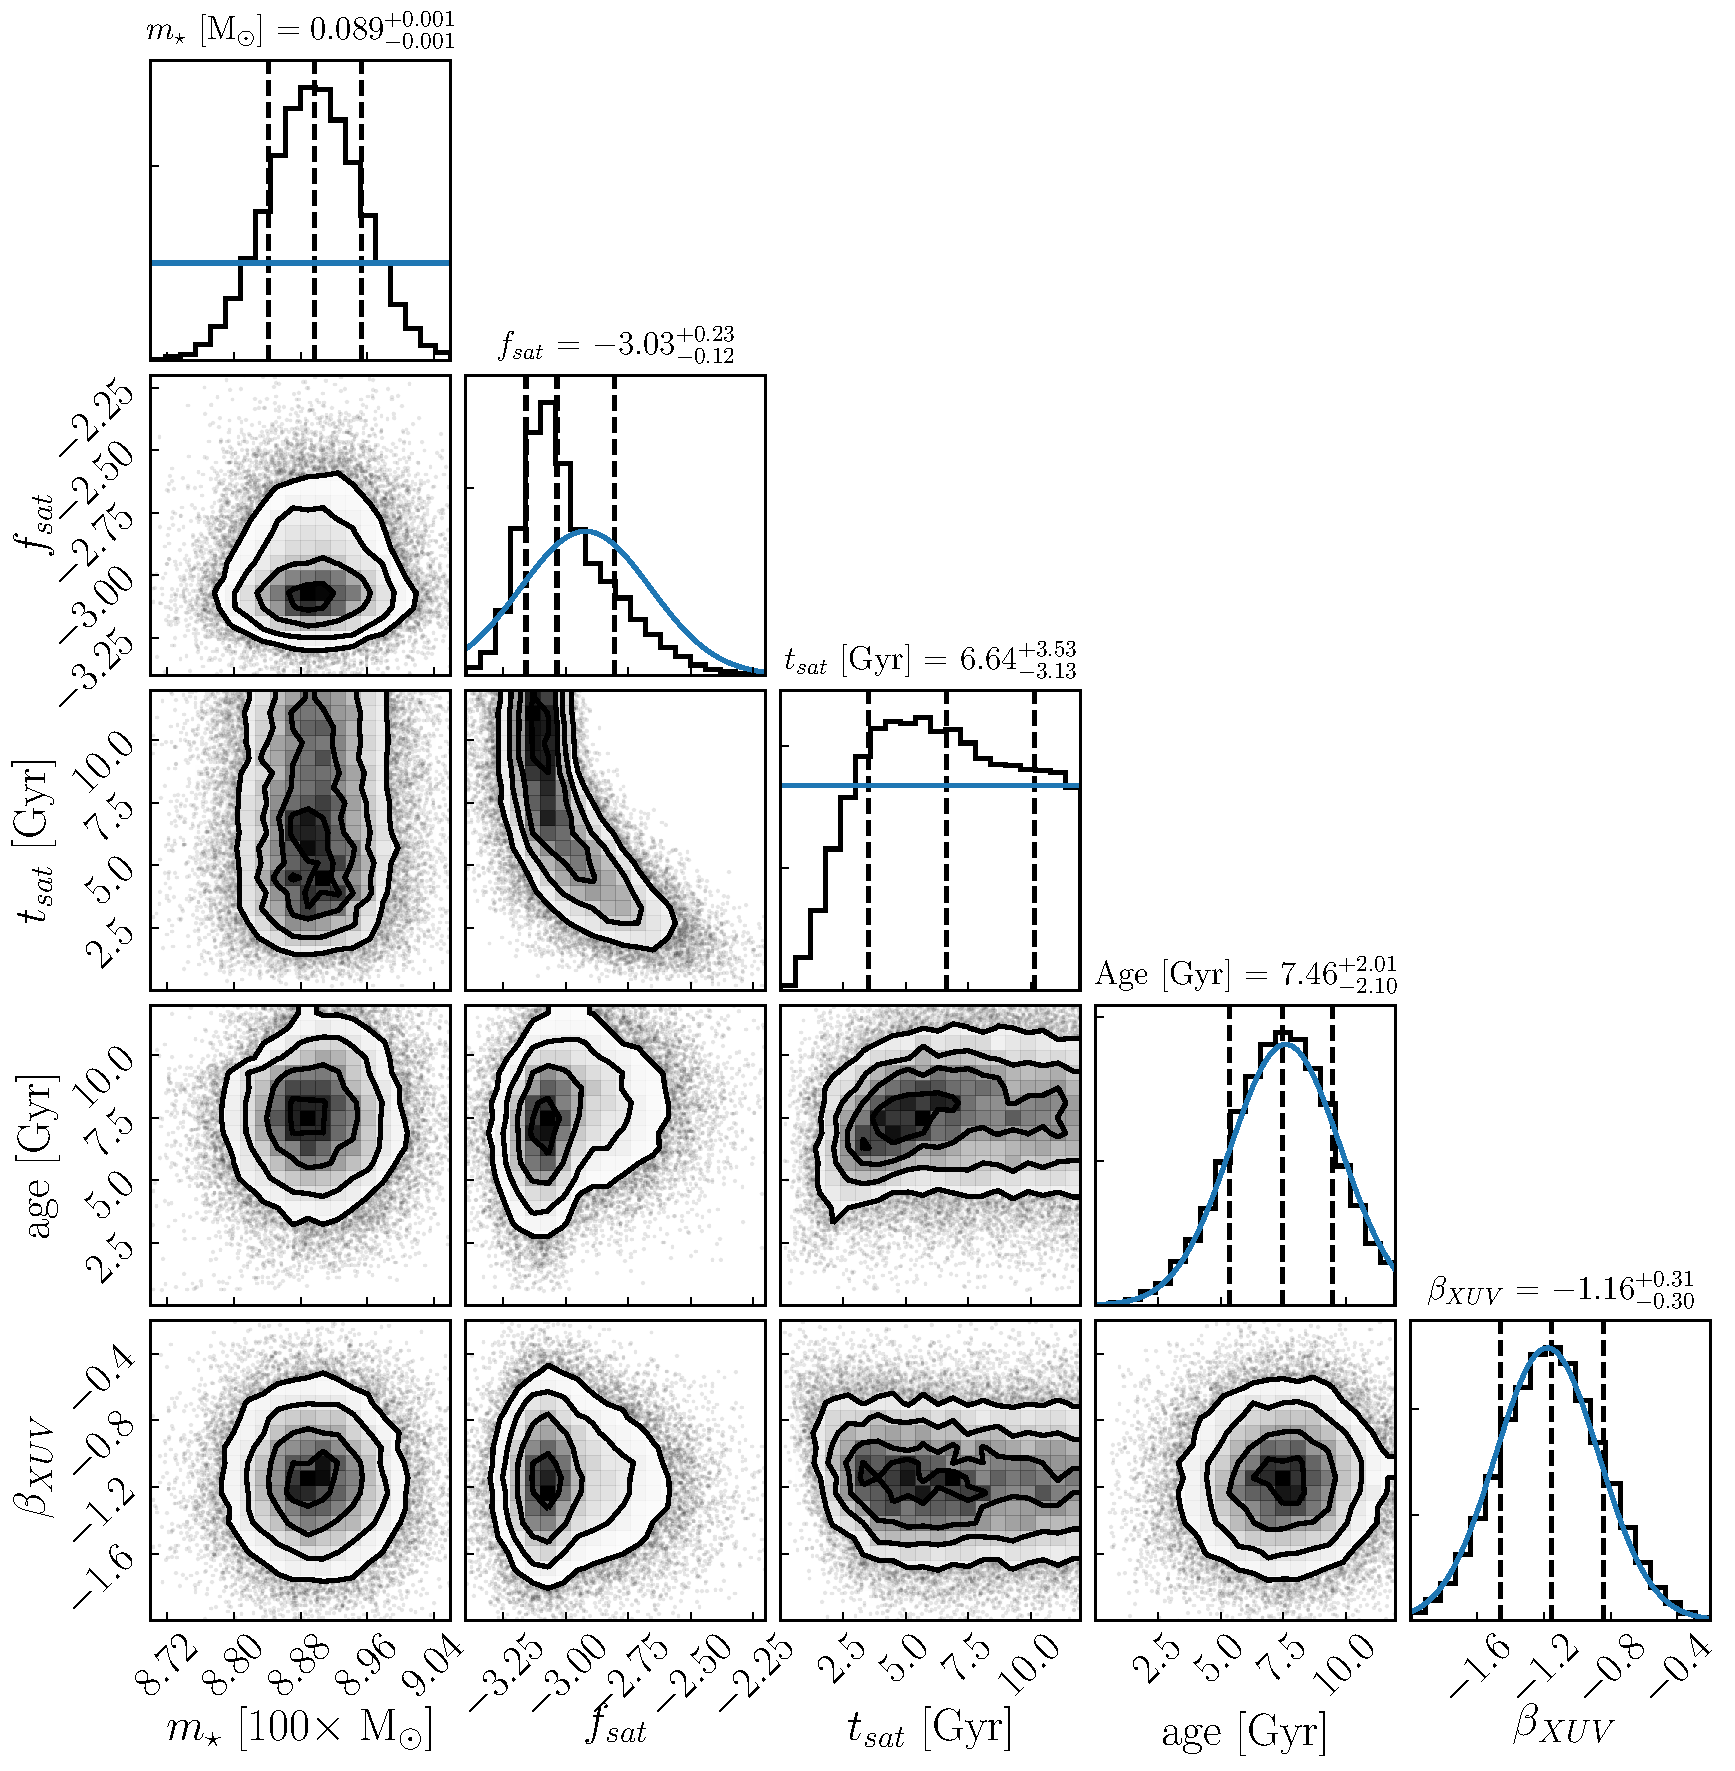
\includegraphics[width=\textwidth]{trappist1Corner.pdf}
   \caption{Joint and marginal posterior probability distributions for the TRAPPIST-1 stellar parameters given in Eqn.~(\ref{trap:eqn:state}) made using \texttt{corner} \citep{ForemanMackey2016}. The black vertical dashed lines on the marginal distributions indicate the median values and lower and upper uncertainties from the 16th and 84th percentiles, respectively. The blue curves superimposed on the marginal distributions display the adopted prior probability distribution for each parameter. From the posterior, I infer that there is a $40\%$ chance that TRAPPIST-1 is still in the saturated phase today.}%
    \label{trap:fig:corner}%
\end{figure*}

The marginal age and $\beta_{XUV}$ posterior distributions reflect their prior distributions as for the former, $L_{bol}$ is not sufficient to constrain TRAPPIST-1's age beyond the adopted prior because the luminosities of ultracool dwarfs do not significantly change during the main sequence \citep{Baraffe2015}. The marginal posterior for $\beta_{XUV}$ does not vary from the prior because the XUV model is over-parameterized with 3 parameters to fit 2 observations, although all are motivated by empirical data and hence merit inclusion. My model prefers to exploit the degeneracy between $f_{sat}$ and $t_{sat}$ to match TRAPPIST-1's observed $L_{XUV}$ in the MCMC instead of varying the slope of the unsaturated $L_{XUV}$ decay. Even though the model is over-parameterized, the observations of TRAPPIST-1 used to condition the probabilistic model do in fact influence the posterior distribution as the reduction in posterior variance relative to the prior can be seen in the joint posterior and marginal distributions of Fig.~\ref{trap:fig:corner} for $m_{\star}$, $f_{sat}$, and $t_{sat}$.

In the joint posterior distribution, age and $\beta_{XUV}$ weakly correlate with $f_{sat}$, requiring a narrow spread of $f_{sat} \approx -3.05$ for young ages and steeper $\beta_{XUV}$, respectively. $\beta_{XUV}$ and $t_{sat}$ are uncorrelated, except at short $t_{sat}$ where steep $\beta_{XUV}$ are disfavored as this evolution would underpredict the observed $L_{XUV}$. I constrain TRAPPIST-1's mass to $m_{\star} = 0.089 \pm{0.001}$ M$_{\odot}$, in a good agreement with and $6\times$ more precise than the value derived by \citet{vanGrootel2018}. In $\S$~\ref{trap:sec:evol}, I consider how this mass constrain impacts TRAPPIST-1's predicted radius.

Finally, I estimate the Monte Carlo standard error (MCSE) for each model parameter. The MCSE does not reflect the inherent probabilistic uncertainty in the model that arises from conditioning on data with uncertainties, but rather it approximates the error incurred by estimating parameters using an ensemble of MCMC chains of finite length. Using the batch means method \citep{Flegal2008,Flegal2010}, I find MCSEs for $m_{\star}$, $f_{sat}$, $t_{sat}$, age, and $\beta_{XUV}$ of $3.41 \times 10^{-6}$, $1.23 \times 10^{-3}$, $2.0 \times 10^{-2}$, $1.30 \times 10^{-2}$, and $2.12 \times 10^{-3}$, respectively. These errors are much less than the posterior uncertainty and can be safely ignored.

%% approxposterior %%

\subsection{Comparison with \approxposterior} \label{trap:sec:approx}

% Extra
%If using a slower model than ours, perhaps one that models stellar evolution by interpolating tracks over mass, age, and metallicity to additionally constrain [Fe/H], or if testing alternate models of $L_{XUV}$ evolution for model comparisons, the computational expense will grow, exacerbating this issue.

\begin{figure*}
\centering
	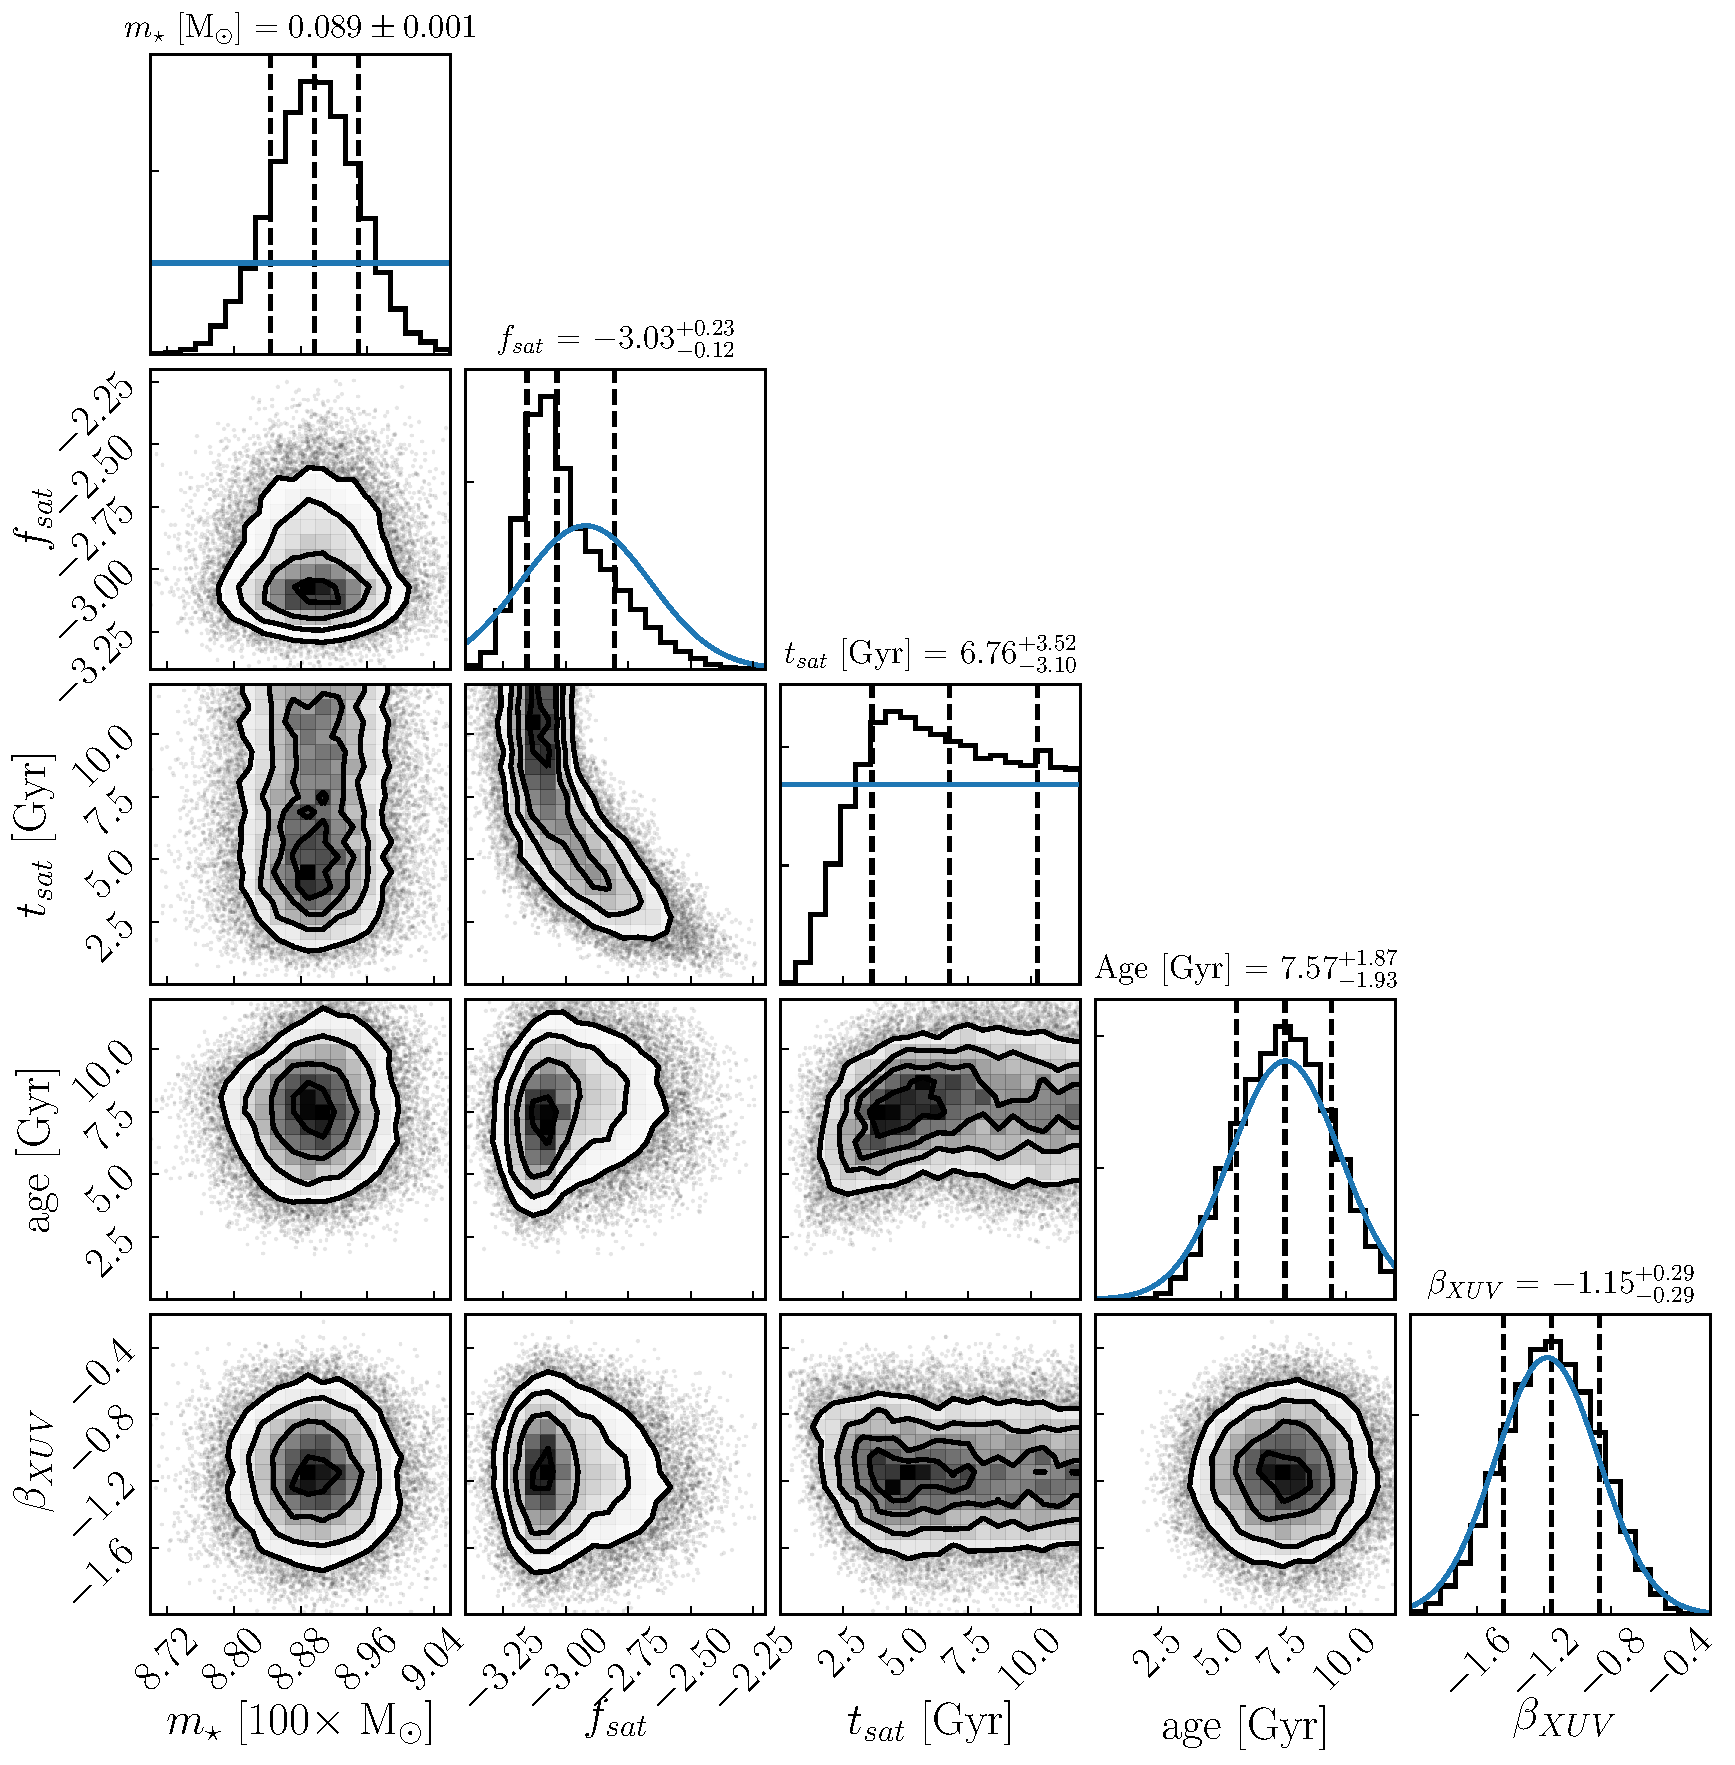
\includegraphics[width=\textwidth]{apCorner.pdf}
   \caption{Same format as Fig.~\ref{trap:fig:corner}, but derived by \approxposterior. \approxposterior recovered constraints and parameter correlations that are in good agreement with the \emcee MCMC, but requiring $980\times$ less computational resources.}%
    \label{trap:fig:approx}%
\end{figure*}

I compare the approximate posterior distribution derived using \approxposterior with my previous results discussed above (referred to as the fiducial MCMC). I display the approximate joint and marginal posterior distributions in Fig.~\ref{trap:fig:approx} and list the marginal constraints derived by both methods in Table~\ref{trap:tab:constraints}.

As seen in Fig.~\ref{trap:fig:approx}, \approxposterior recovers the non-trivial correlations between model parameters seen in the fiducial MCMC posterior distribution. I emphasize this good agreement by overplotting the \approxposterior estimated posterior distribution (blue) on top of the fiducial MCMC results (black) in Fig.~\ref{trap:fig:stacked}.

The parameter constraints derived using \approxposterior are in good agreement with those inferred using \emcee. I find average errors in parameter medians and $1\sigma$ uncertainties of $0.61\%$ and $5.5\%$, respectively, relative to the constraints deriving using \emcee. These differences are larger than the MCSEs because the GP employed by \approxposterior is an accurate, yet imperfect, surrogate for the lnprobability calculation. \approxposterior tends to underestimate parameter uncertainties by a few percent because its algorithm preferentially selects high-likelihood points to expand its training set (see $\S$~\ref{AP:sec:augment}). This concentration of high-likelihood points slightly biases the inferred GP scale lengths, $l$, towards smaller values, effectively overfitting. The smaller values of $l$ shrink the estimated posterior distribution, producing the underestimated parameter uncertainties. I mitigate this effect by adding a small white noise term to the diagonal of the GP covariance matrix.

Not only can \approxposterior accurately recover Bayesian parameter constraints and correlations, it does so extremely quickly. \approxposterior requires only about 4 core hours to estimate the approximate posterior distribution, a factor of $980\times$ faster than the fiducial MCMC. Moreover, \approxposterior used $1330\times$ fewer \vplanet simulations to build its training set than the ${\sim}10^6$ simulations ran by the fiducial MCMC for likelihood evaluations. This reduction in computational expense arises from a combination of \approxposterior's GP-based lnprobability predictions only taking ${\sim}130\mu$s, compared to the much longer $10$s per \vplanet simulation, and its intelligent iterative training set augmentation algorithm. \approxposterior's efficient selection of the GP's training set focuses on high-likelihood regions to improve the GP's predictive ability in relevant regions of parameter space while minimizing the training set size.

\begin{figure*}
\centering
	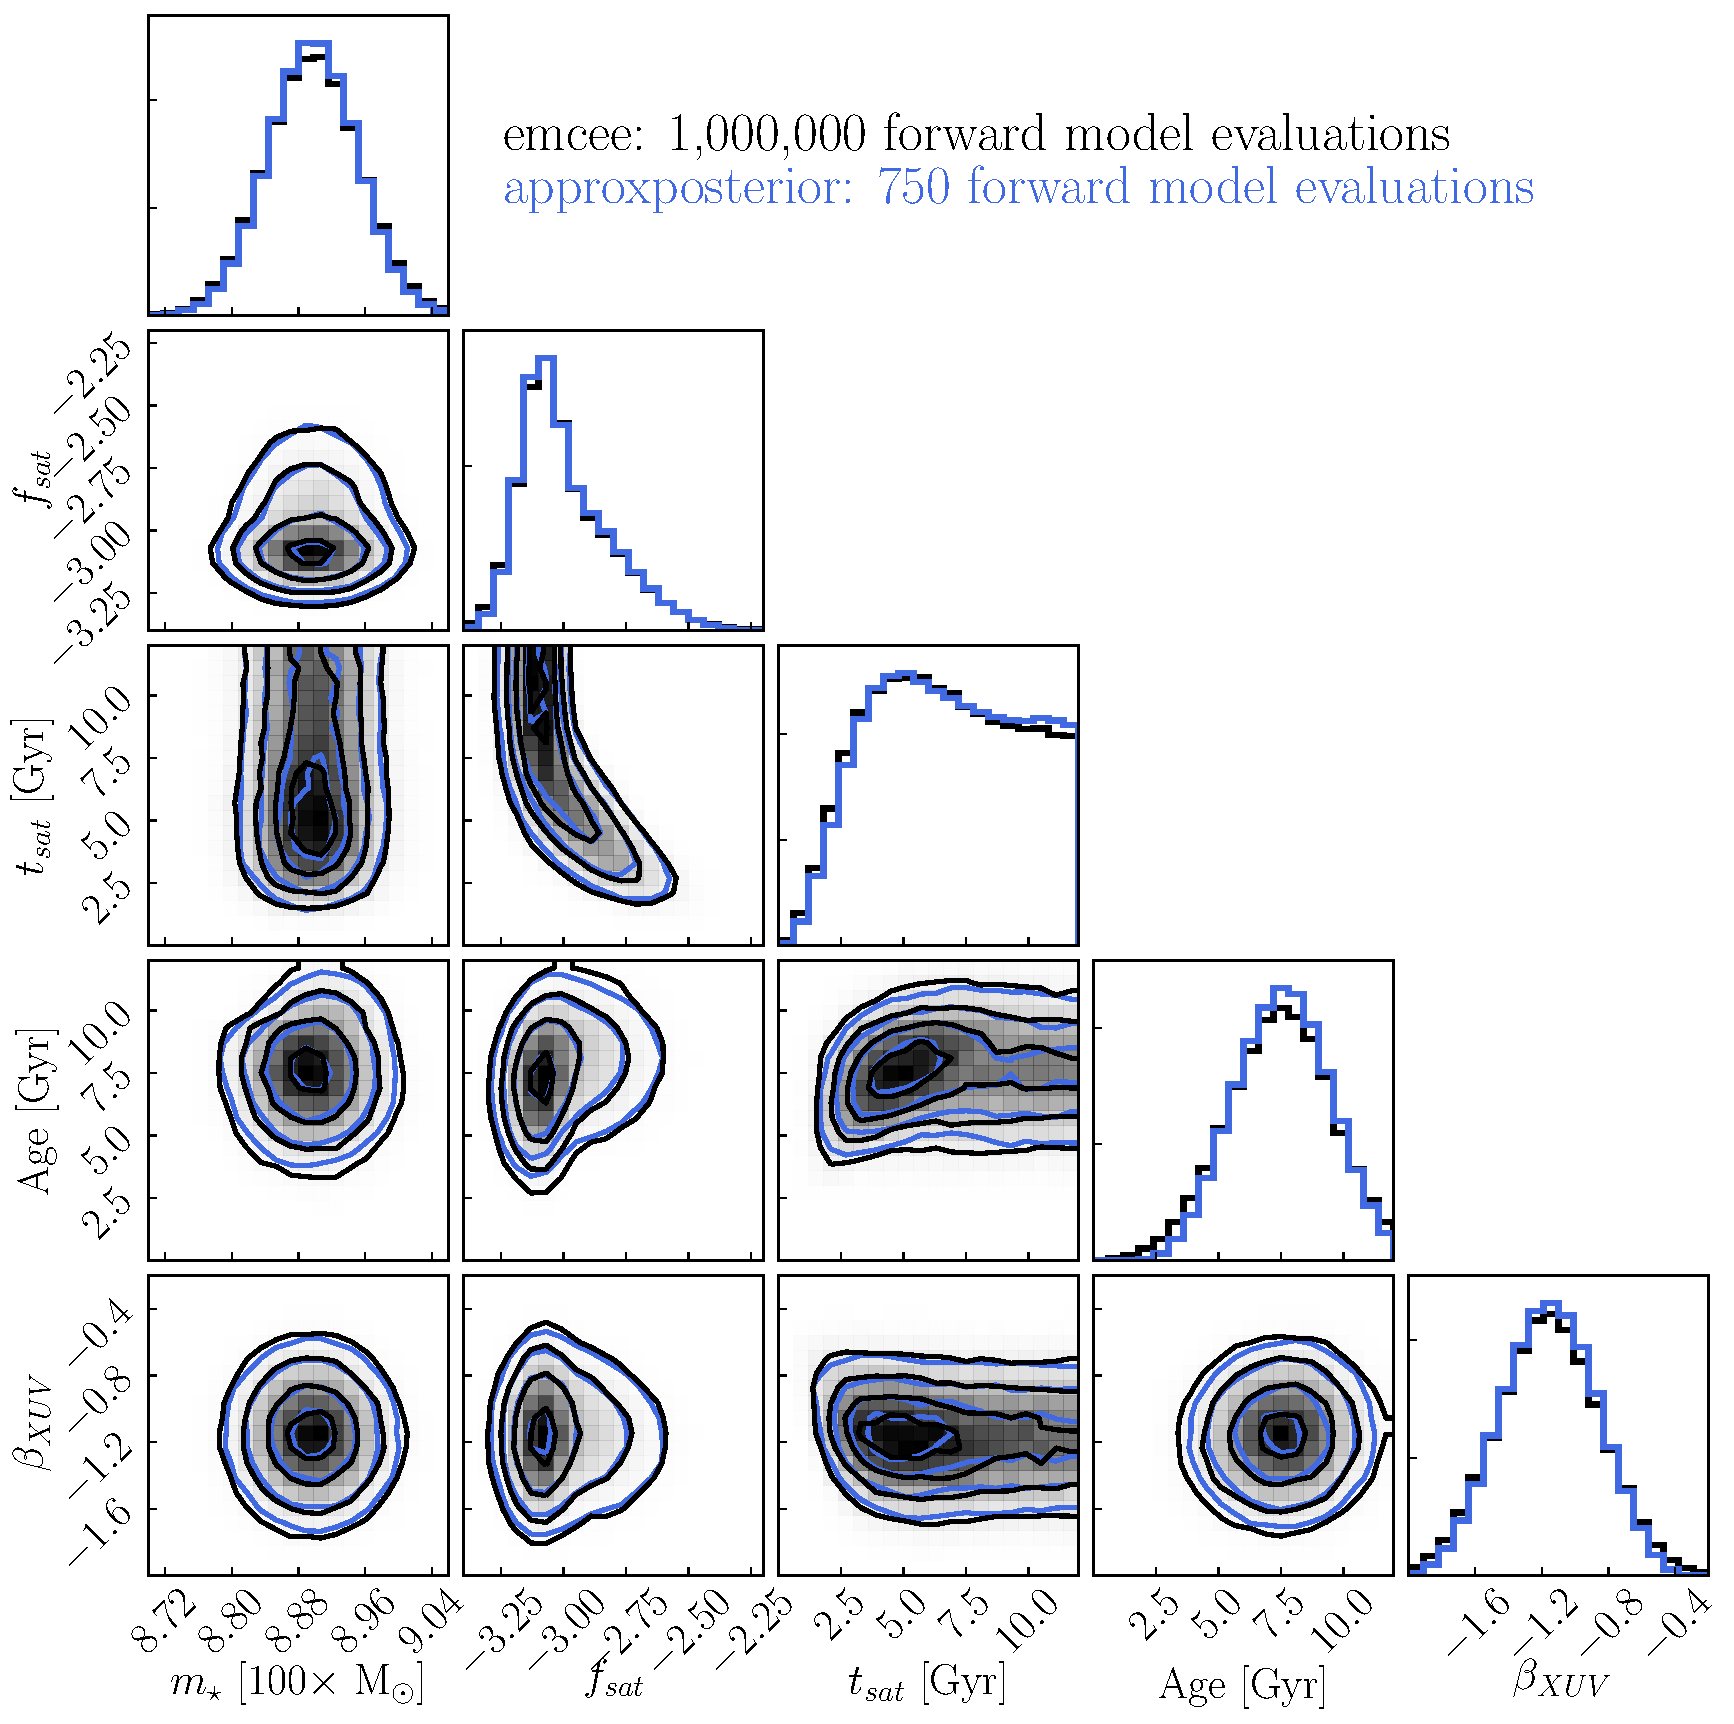
\includegraphics[width=\textwidth]{stacked.pdf}
   \caption{Same format as Fig.~\ref{trap:fig:corner}, but with the fiducial posterior distribution in black and the \approxposterior-derived posterior distribution in blue. The joint and marginal posterior distributions estimated by \approxposterior are in excellent agreement with the fiducial \emcee-derived results.}%
    \label{trap:fig:stacked}%
\end{figure*}

My findings demonstrate that \approxposterior can be used to estimate accurate approximations to the posterior probability distributions of the parameters that control stellar XUV evolution in late M dwarfs, but significantly faster than traditional MCMC methods. Note that \approxposterior is agnostic to the underlying forward model it learns on, enabling Bayesian parameter inference with other computationally-expensive forward models.

% deprecated
% The posterior distribution derived by \approxposterior, however, is not an exact match. \approxposterior underestimates the magnitude of both the age and $\beta_{XUV}$ uncertainties by ${\sim}30\%$ and predicts that there is a $39\%$ chance that TRAPPIST-1 is still saturated today, $9\%$ smaller than the fiducial MCMC-derived value.

\begin{deluxetable}{lcccc}
\tabletypesize{\small}
\tablecaption{Parameter Constraints and Errors \label{trap:tab:constraints}} 
\tablehead{
\colhead{Parameter [units]} & \colhead{\vplanet-\emcee MCMC} & \colhead{AP MCMC} & \colhead{AP Relative Error} & \colhead{Monte Carlo Error}
}
\startdata
$m_\star$ [$M_{\odot}$] & $0.089^{+0.001}_{-0.001}$ &  $0.089^{+0.001}_{-0.001}$ & ${<}0.1\%$ & $3.41\times 10^{-6}$ \\  
$f_{sat}$ & $-3.03^{+0.23}_{-0.12}$ & $-3.03^{+0.23}_{-0.12}$ & ${<}0.1\%$ & $1.23\times 10^{-3}$  \\
$t_{sat}$ [Gyr] & $6.64^{+3.53}_{-3.13}$ & $6.76^{+3.52}_{-3.10}$ & $1.81\%$ & $2.0\times 10^{-2}$ \\
age [Gyr] & $7.46^{+2.01}_{-2.10}$ & $7.57^{+1.87}_{-1.93}$ & $1.47\%$ & $1.30 \times 10^{-3}$ \\
$\beta_{XUV}$ & $-1.16^{+0.31}_{-0.30}$ & $-1.15^{+0.29}_{-0.29}$ & $0.86\%$ & $2.12\times 10^{-3}$ \\
P$(\mathrm{saturated})$ & $0.40$ & $0.39$ & $2.5\%$ & $3.30 \times 10^{-3}$ \\
\enddata \vspace*{0.1in}
\tablecomments{Best fit values and uncertainties are derived using the medians, $16^{th}$, and $84^{th}$ percentiles from the marginal posterior distributions, respectively. Here, AP is shorthand for \approxposterior. P$(\mathrm{saturated})$ indicates the posterior probability that TRAPPIST-1 is still in the saturated regime today. The relative errors are computed as the absolute percent difference between the best fit values derived by \emcee and \approxposterior. The \approxposterior-derived results are in good agreement with the fiducial \emcee MCMC.}
\end{deluxetable}

\subsection{TRAPPIST-1's Evolutionary History and Its Planets' XUV Environment} \label{trap:sec:evol}

I consider plausible stellar evolutionary histories for TRAPPIST-1 by simulating 100 samples from the posterior distribution. I plot the evolution of TRAPPIST-1's $L_{bol}$, $L_{XUV}$, and radius in Fig.~\ref{trap:fig:evol} and compare my models to the measured values. 

\begin{figure*}
	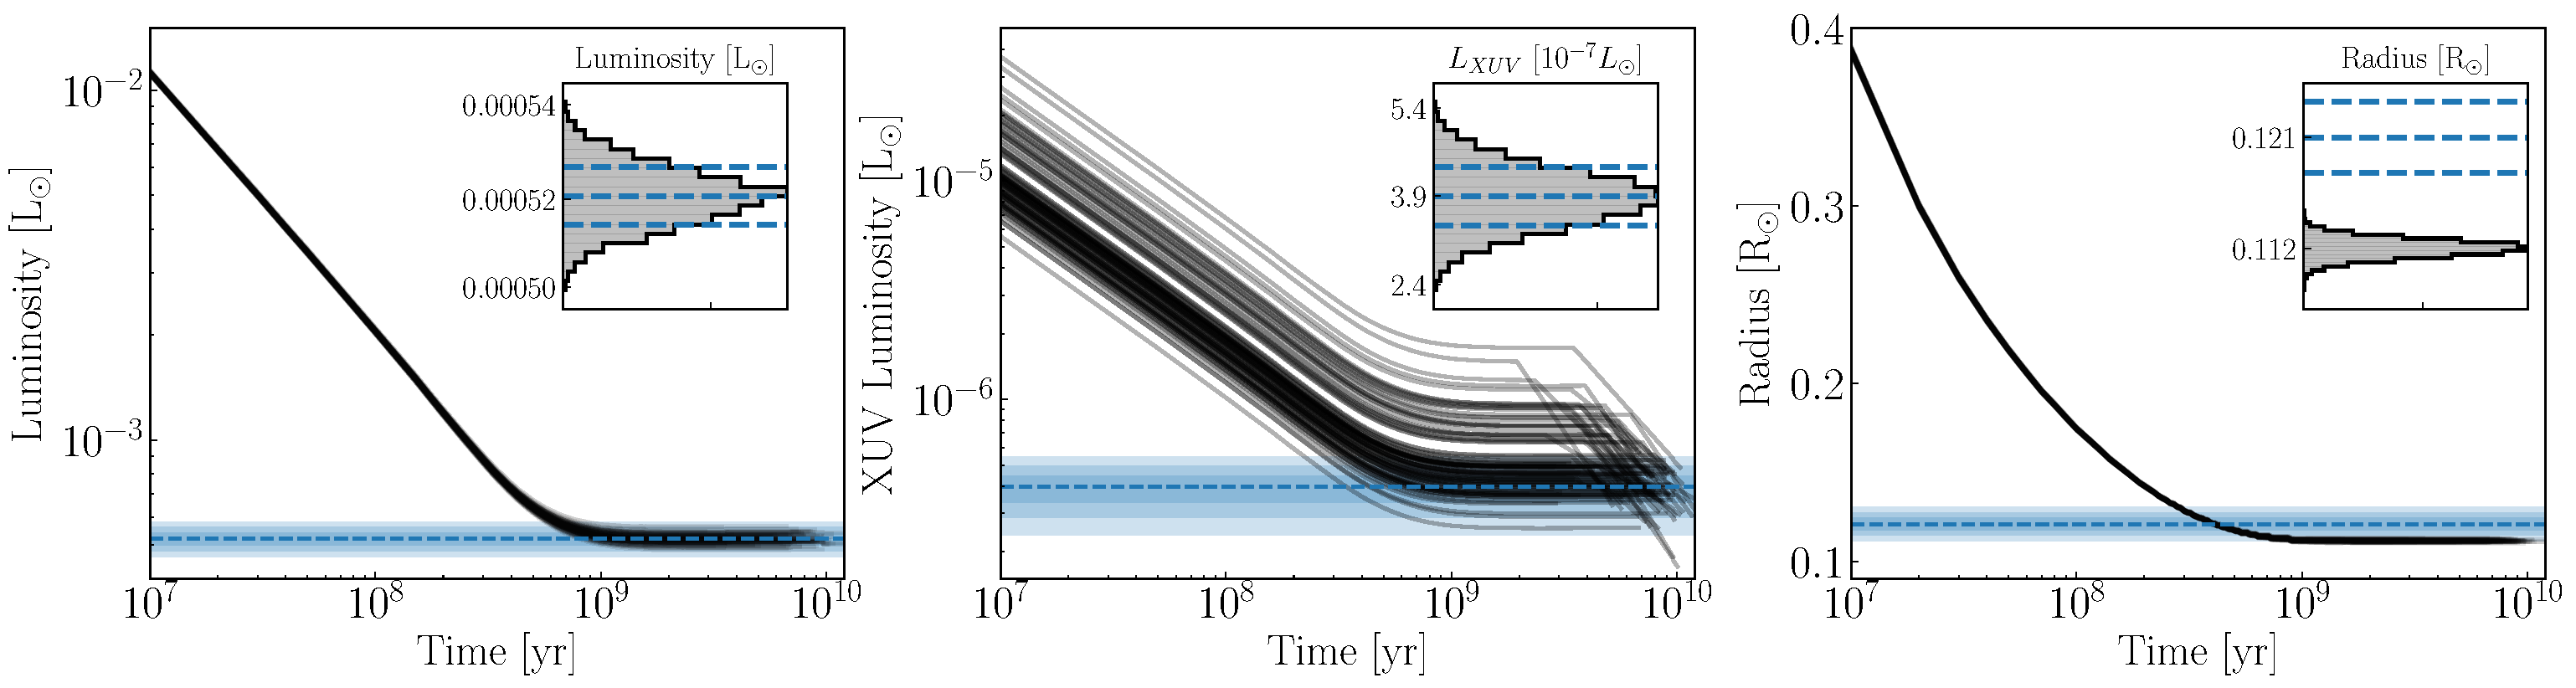
\includegraphics[width=\textwidth]{trappist1Evol.pdf}
   \caption{Plausible evolutionary histories of TRAPPIST-1's $L_{bol}$ (left), $L_{XUV}$ (center), and radius (right) using 100 samples drawn from the posterior distribution and simulated with \vplanet. In each panel, the blue shaded regions display the 1, 2, and 3 $\sigma$ uncertainties. The insets display the marginal distributions (black) evaluated at the age of the system, with the blue dashed lines indicating the observed value and +/- 1 $\sigma$ uncertainties. The radius, $L_{bol}$, and $L_{XUV}$ constraints are adopted from \citet{vanGrootel2018} and \citet{Wheatley2017}, respectively, by convolving the \citet{vanGrootel2018} $L_{bol}$ measurement with the $L_{XUV}/L_{bol}$ constraints from \citet{Wheatley2017}.}%
    \label{trap:fig:evol}%
\end{figure*}

TRAPPIST-1 remains saturated throughout its $1$ Gyr-long pre-main sequence, with both $L_{XUV}$ and $L_{bol}$ decreasing by a factor of ${\sim}40$ before stabilizing on the main sequence. TRAPPIST-1's radius likely shrank by roughly a factor of 4 along the pre-main sequence. I derive a present-day radius $R_{\star} = 0.112 \pm{0.001} \ R_{\odot}$ from the posterior distribution, a value that is ${\sim} 7\%$ smaller than the \citet{vanGrootel2018} constraint, $R_{\star} = 0.121 \pm {0.003} \ R_{\odot}$, that was computed from their inferred mass and TRAPPIST-1's density \citep{Delrez2018}. This difference arises from the likely underprediction of TRAPPIST-1's radius by the \citet{Baraffe2015} models, consistent with stellar evolution models often underestimating the radii of late M dwarfs \citep{Reid2005,Spada2013}. 

An alternate explanation to account for its inflated radius is that TRAPPIST-1 has super-solar metallicity \citep{Burgasser2017,vanGrootel2018}, but \citet{vanGrootel2018} found in their modeling that TRAPPIST-1 required a metallicity of [Fe/H] = 0.4 to reproduce its density and radius. \citet{vanGrootel2018} show that as this result is $4.5\sigma$ off from the best fit value from \citet{Gillon2016}, who found [Fe/H] $= 0.04 \pm{0.08}$. The super-solar hypothesis is therefore strongly disfavored by the observational data. If I instead compute the radius from the marginal stellar mass posterior distribution and the observed density \citep{Delrez2018}, I obtain $R_{\star} = 0.120 \pm{0.002} \ R_{\odot}$, in agreement with \citet{vanGrootel2018} who used the same procedure.

Since TRAPPIST-1 could still be saturated today, its planetary system has likely experienced a persistent extreme XUV environment. In Fig.~\ref{trap:fig:fluxes}, I probe the distribution of XUV fluxes, $F_{XUV}$, derived from the posterior distributions for each TRAPPIST-1 planet when the system was 0.01, 0.1, and 1 Gyr old. I normalize these values by the $F_{XUV}$ received by Earth during the mean solar cycle \citep[$F_{XUV,\oplus} = 3.88$ erg s$^{-1}$cm$^{-2}$,][]{Ribas2005} and assume the planets remained near their current semi-major axes after migration in the natal protoplanetary disk halted \citep{Luger2017}. 

I infer that TRAPPIST-1b likely received extreme $F_{XUV}/F_{XUV, \oplus} \gsim 10^4$ during the early pre-main sequence before decaying to the present-day $F_{XUV}/F_{XUV, \oplus} \approx 10^3$, consistent with estimates from \citet{Wheatley2017}. The extended upper-tail of the $F_{XUV}$ distributions corresponds to the large $f_{sat}$ values permitted by the posterior distributions. The likely habitable zone planets, e, f, and g, similarly experienced severe XUV fluxes ranging from $F_{XUV}/F_{XUV, \oplus} \approx 10^2 - 10^{3.5}$ throughout the pre-main sequence. Even today, e, f, and g receive $F_{XUV}/F_{XUV, \oplus} \approx 10^2$, far in excess of the modern Earth, due to TRAPPIST-1's large present $L_{XUV}$, its extended saturated phase, and the close proximity of M dwarf HZ planets to their host star. These significant high energy fluxes likely drove an extended epoch of substantial atmospheric escape and water loss from the TRAPPIST-1 planets, potentially producing substantial abiotic O$_2$ atmospheres \citep{Luger2015,Bolmont2017,Bourrier2017a}.

\begin{figure}
	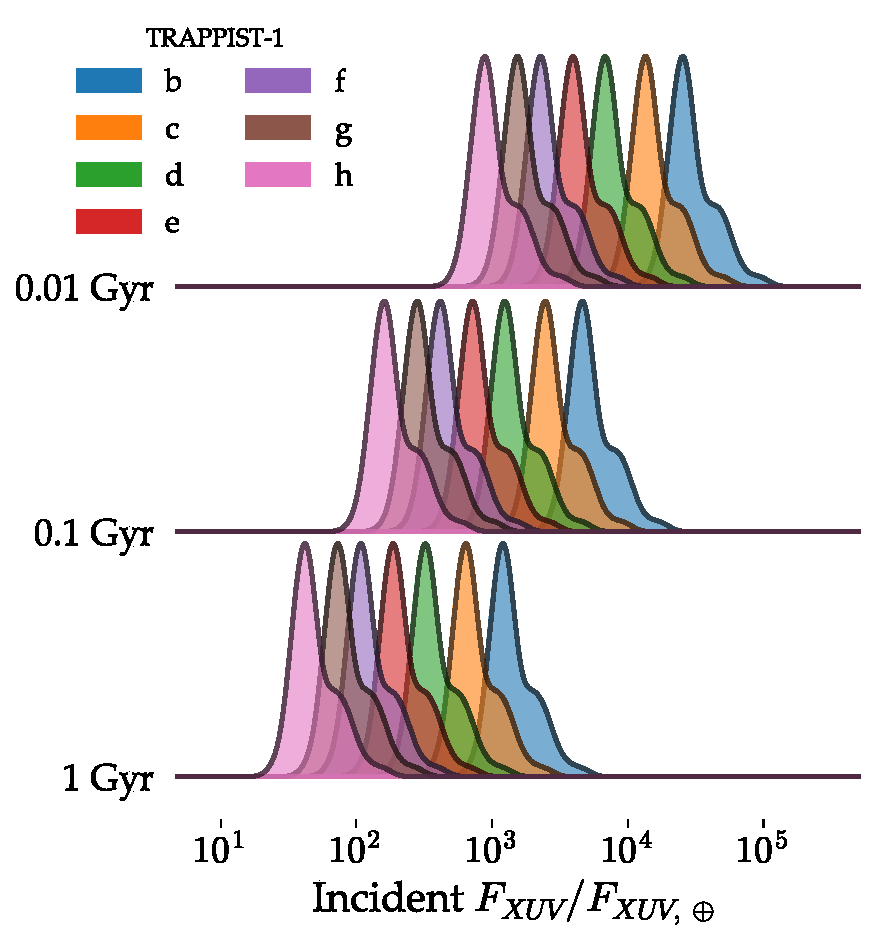
\includegraphics[width=\textwidth]{fluxes.pdf}
   \caption{$F_{XUV}/F_{XUV,\oplus}$ for each TRAPPIST-1 planet derived from samples drawn from the posterior distribution and simulated using \vplanet when the system was 0.01, 0.1, and 1 Gyr old. The latter age corresponds to the approximate age at which TRAPPIST-1 entered the main sequence. The TRAPPIST-1 planetary system has likely endured a long-lasting extreme XUV environment.}%
    \label{trap:fig:fluxes}%
\end{figure}

%% Discussion %%

\section{Discussion and Conclusions} \label{trap:sec:discussion}

In this Chapter, I used MCMC to derive probabilistic constraints for TRAPPIST-1's stellar and $L_{XUV}$ evolution to characterize the evolving XUV environment of its planetary system. I inferred that TRAPPIST-1 likely maintained high $L_{XUV}/L_{bol} \approx 10^{-3}$ throughout its lifetime, with a $40\%$ chance that TRAPPIST-1 is still in the saturated regime today. My results indicate that at least some ultracool dwarfs can sustain large $L_{XUV}$ in the saturated regime for Gyrs, consistent with activity lifetimes of late M dwarfs \citep{West2008}. I suggest that studies of volatile loss from planets orbiting ultracool dwarfs model the long-term $L_{XUV}$ evolution of the host star, or at least assume saturation timescales of $t_{sat}{\gsim}4$ Gyrs. My choice of prior distributions strongly impacts my results as the inference hinges on only two measured properties of TRAPPIST-1, $L_{XUV}$ and $L_{bol}$. To mitigate this effect, I consulted previous studies and empirical observations of the activity evolution of late M dwarfs to construct realistic prior distributions.

The TRAPPIST-1 planets likely experienced significant XUV fluxes during the pre-main sequence, potentially driving extreme atmospheric erosion and water loss \citep{Bolmont2017,Bourrier2017a}. The high-energy fluxes incident on the inner-most planets throughout this phase were probably large enough for atmospheric mass loss to be recombination-limited ($F_{UV} \gsim 10^4$ g s$^{-1}$ cm$^{-2}$) and scale as $\dot{m} \sim F_{XUV}^{0.6}$ \citep{MurrayClay2009}, as opposed to the oft-assumed energy-limited escape \citep[$\dot{m} \sim F_{XUV}$,][]{Watson1981,Lammer2003}, potentially inhibiting volatile loss. If the TRAPPIST-1 planets did lose significant amounts of water as my estimates suggest, they must have formed with a large initial volatile inventory to account for their observed low densities \citep{Grimm2018}.

I demonstrated that the open source Python machine learning package, \approxposterior \citep{FlemingVanderPlas2018}, can efficiently compute an accurate approximation to the posterior distribution using an adaptive learning GP-based method, requiring $1330\times$ fewer \vplanet simulations and a factor of $980\times$ less core hours than traditional MCMC approaches. The posterior distributions derived by \approxposterior reproduced the non-trivial parameter correlations and best-fit values uncovered by my fiducial MCMC analysis. I find that \approxposterior recovers the best-fit values and $1\sigma$ uncertainties of the model parameters with an average error of $0.61\%$ and $5.5\%$, respectively, relative to the constraints derived using \emcee. If future observations of TRAPPIST-1 refine its fundamental parameters, and possibly $L_{XUV}/L_{bol}$, \approxposterior can be used to rapidly and accurately replicate this analysis to update the constraints.  

% Extra
% \xxx{Applying these methods to other M dwarfs, however, requires measuring their current $L_{X}$ or $L_{XUV}$, a difficult task given that most M and ultracool dwarfs are faint and that much of the stellar EUV radiation is absorbed by neutral interstellar hydrogen \citep{Airapetian2019}. These quantities, however, can be reconstructed via empirical scaling relations \citep[e.g.][]{Linsky2014}. The accuracy and massive reduction in compute time afforded by \approxposterior enables our analysis to scale to a larger sample of late M dwarfs to constrain their XUV histories.}

I conclude this Chapter by thanking the anonymous referee for their careful reading of the manuscript that became this Chapter. This work was facilitated though the use of advanced computational, storage, and networking infrastructure provided by the Hyak supercomputer system and funded by the Student Technology Fund at the University of Washington. DPF was supported by NASA Headquarters under the NASA Earth and Space Science Fellowship Program - Grant 80NSSC17K0482.  This work was supported by the NASA Astrobiology Program Grant Number 80NSSC18K0829 and benefited from participation in the NASA Nexus for Exoplanet Systems Science research coordination network. For this Chapter, I used the following software: \approxposterior: \citet{FlemingVanderPlas2018}, \texttt{corner}: \citet{ForemanMackey2016}, \texttt{emcee}: \citet{ForemanMackey2013}, \texttt{george}: \citet{george}, and \vplanet: \citet{Barnes2019}
